\documentclass{beamer}
\mode<presentation> {
\usepackage{color}
\definecolor{bottomcolour}{rgb}{0.21,0.11,0.21}
\definecolor{middlecolour}{rgb}{0.21,0.11,0.21}
\setbeamercolor{structure}{fg=white}
\setbeamertemplate{frametitle}[default]%[center]
\setbeamercolor{normal text}{bg=black, fg=white}
\setbeamertemplate{background canvas}[vertical shading]
[bottom=bottomcolour, middle=middlecolour, top=black]
\setbeamertemplate{items}[circle]
\setbeamertemplate{navigation symbols}{} %no nav symbols
\setbeamercolor{block title}{use=structure,fg=white,bg=structure.fg!50!red!50!blue!100!green}
\setbeamercolor{block body}{parent=normal text,use=block title,bg=block title.bg!5!white!10!bg,fg=white}
\setbeamertemplate{navigation symbols}{}
}
\usepackage{graphicx} 
\usepackage{booktabs} 
\usepackage[utf8]{inputenc}  
\usepackage[T1]{fontenc}  
\usepackage{geometry}     
%\usepackage[francais]{babel} 
\usepackage{eurosym}
\usepackage{verbatim}
\usepackage{ragged2e}
\justifying

%%%%%%%%%%%%%%%%%%%%%%%%%%%%%%%%%%%%%%%%%%%%%%%%%%%%%%%%%%%%%%%%
%% ccBeamer 0.1, 2007-07-02                                   %%
%% Written by Sebastian Pipping <webmaster@hartwork.org>      %%
%% ---------------------------------------------------------- %%
%% Licensed under Creative Commons Attribution-ShareAlike 3.0 %%
%% http://creativecommons.org/licenses/by-sa/3.0/             %%
%%%%%%%%%%%%%%%%%%%%%%%%%%%%%%%%%%%%%%%%%%%%%%%%%%%%%%%%%%%%%%%%


%% Images
\newcommand{\CcImageBy}[1]{%
	
\includegraphics[scale=#1]{creative_commons/cc_by_30.pdf}%
}
\newcommand{\CcImageCc}[1]{%
	
\includegraphics[scale=#1]{creative_commons/cc_cc_30.pdf}%
}
\newcommand{\CcImageDevNations}[1]{%
	
\includegraphics[scale=#1]{creative_commons/cc_dev_nations_30.pdf}%
}
\newcommand{\CcImageNc}[1]{%
	
\includegraphics[scale=#1]{creative_commons/cc_nc_30.pdf}%
}
\newcommand{\CcImageNd}[1]{%
	
\includegraphics[scale=#1]{creative_commons/cc_nd_30.pdf}%
}
\newcommand{\CcImagePd}[1]{%
	
\includegraphics[scale=#1]{creative_commons/cc_pd_30.pdf}%
}
\newcommand{\CcImageSa}[1]{%
	
\includegraphics[scale=#1]{creative_commons/cc_sa_30.pdf}%
}
\newcommand{\CcImageSampling}[1]{%
	
\includegraphics[scale=#1]{creative_commons/cc_sampling_30.pdf}%
}
\newcommand{\CcImageSamplingPlus}[1]{%
	
\includegraphics[scale=#1]{creative_commons/cc_sampling_plus_30.pdf}%
}


%% Groups
\newcommand{\CcGroupBy}[1]{% zoom
	\CcImageBy{#1}%
}
\newcommand{\CcGroupByNc}[2]{% zoom, gap
	\CcImageBy{#1}\hspace*{#2}\CcImageNc{#1}%
}
\newcommand{\CcGroupByNcNd}[2]{% zoom, gap
	\CcImageBy{#1}\hspace*{#2}\CcImageNc{#1}\hspace*{#2}\CcImageNd{#1}%
}
\newcommand{\CcGroupByNcSa}[2]{% zoom, gap
	\CcImageBy{#1}\hspace*{#2}\CcImageNc{#1}\hspace*{#2}\CcImageSa{#1}%
}
\newcommand{\CcGroupByNd}[2]{% zoom, gap
	\CcImageBy{#1}\hspace*{#2}\CcImageNd{#1}%
}
\newcommand{\CcGroupBySa}[2]{% zoom, gap
	\CcImageBy{#1}\hspace*{#2}\CcImageSa{#1}%
}
\newcommand{\CcGroupDevNations}[1]{% zoom
	\CcImageDevNations{#1}%
}
\newcommand{\CcGroupNcSampling}[2]{% zoom, gap
	\CcImageNc{#1}\hspace*{#2}\CcImageSampling{#1}%
}
\newcommand{\CcGroupPd}[1]{% zoom
	\CcImagePd{#1}%
}
\newcommand{\CcGroupSampling}[1]{% zoom
	\CcImageSampling{#1}%
}
\newcommand{\CcGroupSamplingPlus}[1]{% zoom
	\CcImageSamplingPlus{#1}%
}


%% Text
\newcommand{\CcLongnameBy}{Attribution}
\newcommand{\CcLongnameByNc}{Attribution-NonCommercial}
\newcommand{\CcLongnameByNcNd}{Attribution-NoDerivs}
\newcommand{\CcLongnameByNcSa}{Attribution-NonCommercial-ShareAlike}
\newcommand{\CcLongnameByNd}{Attribution-NoDerivs}
\newcommand{\CcLongnameBySa}{Attribution-ShareAlike}

\newcommand{\CcNote}[1]{% longname
	This work is licensed under the \textit{Creative Commons #1 3.0 License}.%
}


\title[Reprenons le contrôle de notre vie privée sur Internet]{Reprenons le contrôle \\de notre vie privée sur Internet
\\~\\

\includegraphics[scale=0.2]{./images/logo-capitole.png}
} 
\date{21-22 novembre 2015}

\author{Genma}

\begin{document}

%% Titlepage
\begin{frame}
	\titlepage
	\vfill
	\begin{center}
		\CcGroupByNcSa{0.83}{0.95ex}\\[2.5ex]
		{\tiny\CcNote{\CcLongnameByNcSa}}
		\vspace*{-2.5ex}
	\end{center}
\end{frame}

\begin{frame}
\frametitle{
\includegraphics[scale=0.4]{./images/Genma.jpg} \ \ \  A propos de moi  }
\begin{columns}[c] 
\column{.55\textwidth} 
\textbf{Où me trouver sur Internet?}
\begin{itemize}
\item Le Blog de Genma : http://genma.free.fr
\item Twitter : http://twitter.com/genma
\end{itemize}
\column{.5\textwidth} 
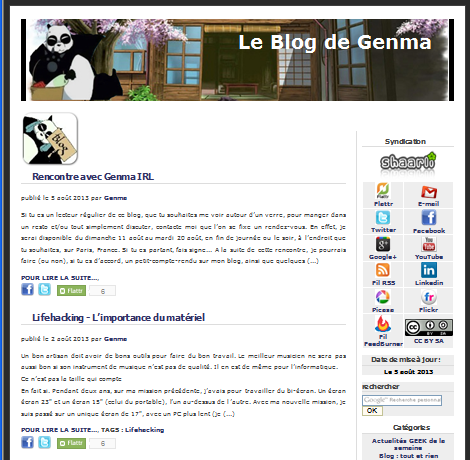
\includegraphics[scale=0.40] {./images/blog.png} 
\end{columns}
\end{frame}

\begin{frame}
\Huge{\centerline{Toutes ces traces qu'on laisse}}
\Huge{\centerline{sur Internet... sans le savoir}}
\end{frame}


%----------------------------------------------------------------------------------------
\begin{frame}
\begin{center}
\Huge{Toutes ces informations \\ que l'on donne... }
\end{center}
\end{frame}

%----------------------------------------------------------------------------------------
\begin{frame}
\frametitle{Diffusion de photos et autres selfies...}
\begin{center}

\includegraphics[scale=0.5] {./images/Leak02.png} 
\end{center}
\end{frame}

%----------------------------------------------------------------------------------------
\begin{frame}
\begin{center}
\Huge{Toutes ces informations \\ que l'on donne... }
\Huge{volontairement...\\~\\ou pas!}
\end{center}
\end{frame}

%----------------------------------------------------------------------------------------
\begin{frame}
\frametitle{Les données qui sont prises à notre insu}

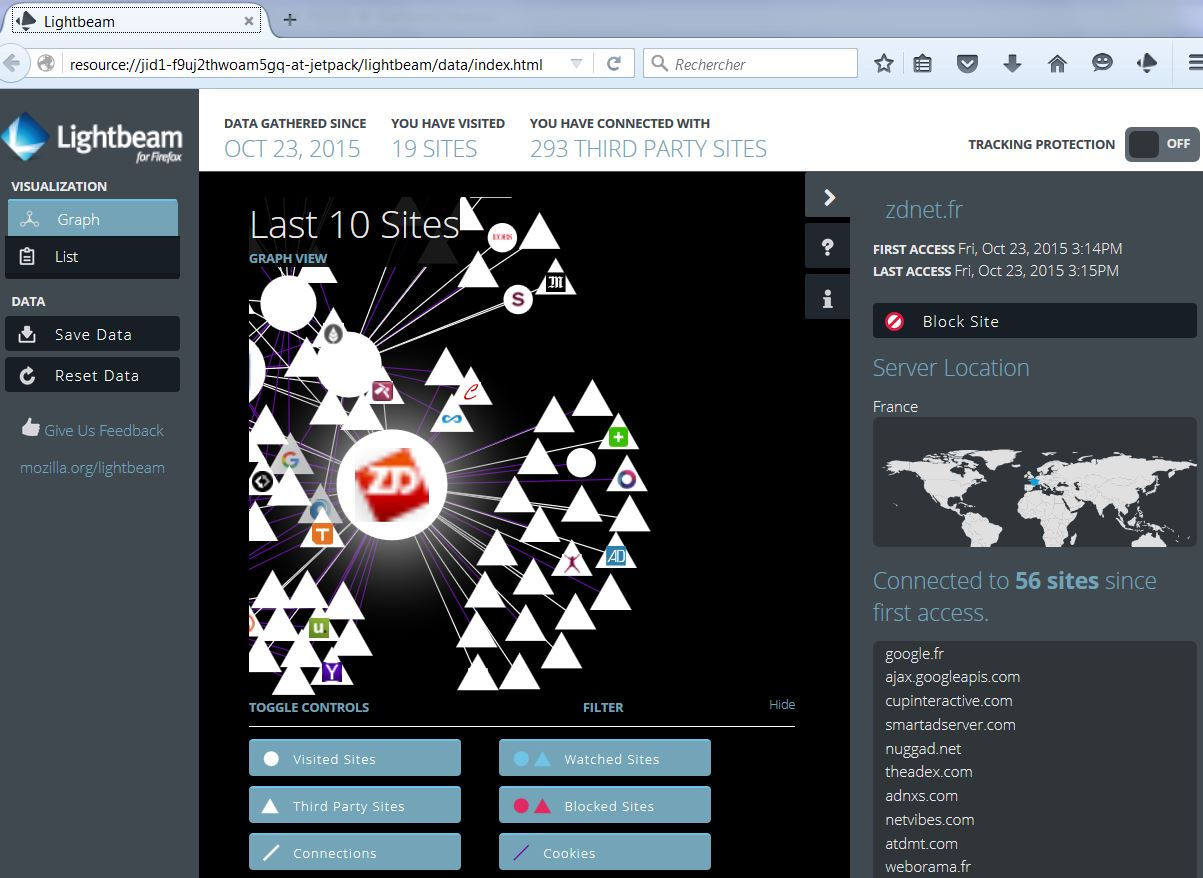
\includegraphics[scale=0.45] {./images/Lightbeam.jpg} 

\end{frame}

%----------------------------------------------------------------------------------------
\begin{frame}
\frametitle{Cloud - l'informatique dans les nuages}
\begin{block}{Définition du cloud}
\justifying{
\begin{itemize}
\item Le \emph{Cloud} , c'est l'ordinateur d'un autre.
\end{itemize}
}
\begin{center}

\includegraphics[scale=0.25] {./images/cloud.png} 
\end{center}
\end{block}
\end{frame}
%----------------------------------------------------------------------------------------

\begin{frame}
\begin{center}
\Huge{LES GAFAMs}\\~\\

\includegraphics[scale=0.5] {./images/gafam.jpg} 
\end{center}
\end{frame}

%----------------------------------------------------------------------------------------
\begin{frame}
\frametitle{Les GAFAM}
\begin{block}{GAFAM : Google, Apple, Facebook, Amazon, Microsoft}
\begin{itemize}
\justifying{
\item Concentration des acteurs d’Internet autour de silos;
\item Une centralisation nuisible (frein à l'innovation);
\item Les utilisateurs de ces services ne contrôlent plus leur vie numérique.
}
\end{itemize}
\end{block}
\end{frame}

%----------------------------------------------------------------------------------------
\begin{frame}
\begin{center}
\Huge{Sur Internet, si c'est gratuit, c'est VOUS le produit }
\end{center}
\end{frame}

%========================================================================================
\begin{frame}
\begin{center}

\includegraphics[scale=0.5] {./images/nothingtohide.png} 
\end{center}
\end{frame}

\begin{frame}
\frametitle{L'espionnage 1/2}
\begin{center}

\includegraphics[scale=0.4]{./images/snowden.png}
\end{center}
\begin{itemize}
\item Snowden et ses révélations (NSA)
\item La loi Renseignement en France...
\end{itemize}
\end{frame}

\begin{frame}
\frametitle{L'espionnage 2/2}
\begin{itemize}
\item Notre voisin
\item Notre "ex"
\item Notre collègue de boulot...
\end{itemize}

\includegraphics[scale=0.55]{./images/nixon.jpg}

\includegraphics[scale=0.4]{./images/girlfriend.jpg}
\end{frame}

\begin{frame}
\frametitle{La différence entre la vie privée et la sécurité en une image}
\begin{center}
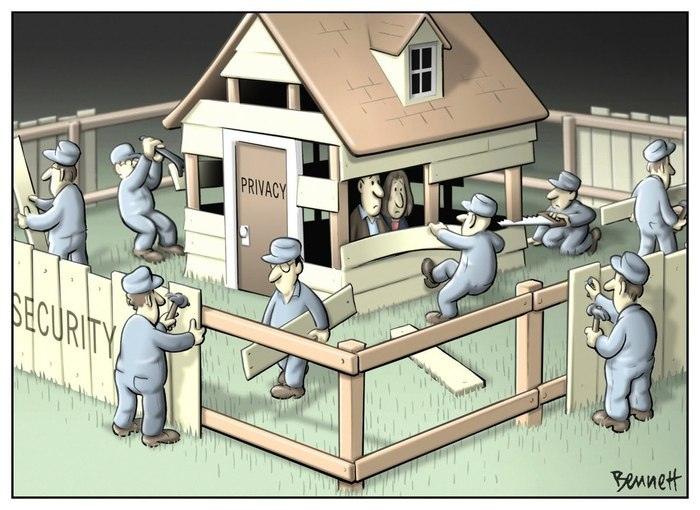
\includegraphics[scale=0.4]{./images/Security_Privacy.jpg}
\end{center}
\end{frame}

%----------------------------------------------------------------------------------------
\begin{frame}
\frametitle{Différents \emph{modèles de menace}}
\begin{block}{Répondre aux questions}
\justifying{
\begin{itemize}
\item Quelles sont les données et informations que j'estime personnelles - confidentielles? 
\item Qu'est ce que je suis prêt-e à apprendre et à faire pour les protéger?
\end{itemize}
}
\end{block}
Pour se faire un avis \url{http://jenairienacacher.fr/}
\end{frame}

%========================================================================================
\begin{frame}
\Huge{\centerline{Comment se protéger ?}}
\Huge{\centerline{Un peu d'hygiène numérique}}
\end{frame}

%----------------------------------------------------------------------------------------
\begin{frame}
\frametitle{L'hygiène numérique?}
\begin{block}{}
\justifying{
L'hygiène est un ensemble de mesures destinées à prévenir les infections et l'apparition de maladies infectieuses.
\\
L'hygiène numérique, ce sont des règles destinées à mieux utiliser son ordinateur, en sécurité, de façon simple.
}
\end{block}
\end{frame}

\begin{frame}
\Huge{\centerline{Quelques exemples?}}
\end{frame}

\begin{frame}
\frametitle{Les règles de sécurité}
\begin{center}
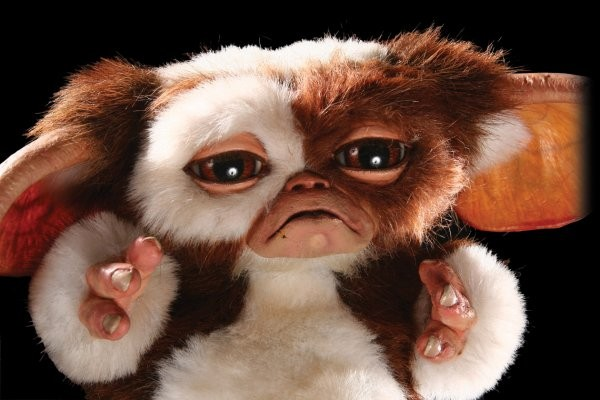
\includegraphics[scale=0.3] {./images/sadgizmo_large.jpeg}
\end{center}

\justifying{
\begin{block}{}
\begin{itemize}
\item Ne pas exposer l'animal à la lumière — et plus spécialement à celle du soleil qui le tuerait, 
\item Ne pas le mouiller, 
\item Et surtout, quoi qu'il arrive, ne jamais lui donner à manger après minuit.
\end{itemize}
\end{block}
}
\end{frame}

\begin{frame}
\Huge{\centerline{Les mots de passe}}
\end{frame}

%----------------------------------------------------------------------------------------
\begin{frame}

\frametitle{Les mots de passe}
\begin{block}{Règles}
\begin{itemize}
\justifying{
\item Plus c'est long, plus c'est bon
\item Ne pas avoir le même mot de passe pour deux comptes en ligne.
}
\end{itemize}
\end{block}

\begin{block}{Mot de passe oublié?}
\justifying{
Pour tester la sécurité d'un site web, on clique sur le lien "mot de passe oublié".
\begin{itemize}
\item Si le mot de passe est renvoyé dans le mail, ce n'est pas bon. Le mot de passe est stocké en "clair".
\end{itemize}
}
\end{block}

\begin{block}{Trop de mot de passe à retenir?}
Il y a le logiciel Keepass. \url{http://www.keepass.info}
\end{block}

\end{frame}

%----------------------------------------------------------------------------------------
\begin{frame}
\begin{center}
\Huge{Navigateur}

\includegraphics[scale=0.4] {./images/firefox.jpg}
\end{center}
\end{frame}

%----------------------------------------------------------------------------------------
\begin{frame}
\begin{center}
\Huge{Installer des extensions \\ pour Firefox }
\end{center}
\end{frame}

%----------------------------------------------------------------------------------------
\begin{frame}
\frametitle{Microblock}
Bloque les publicités.
\begin{center}
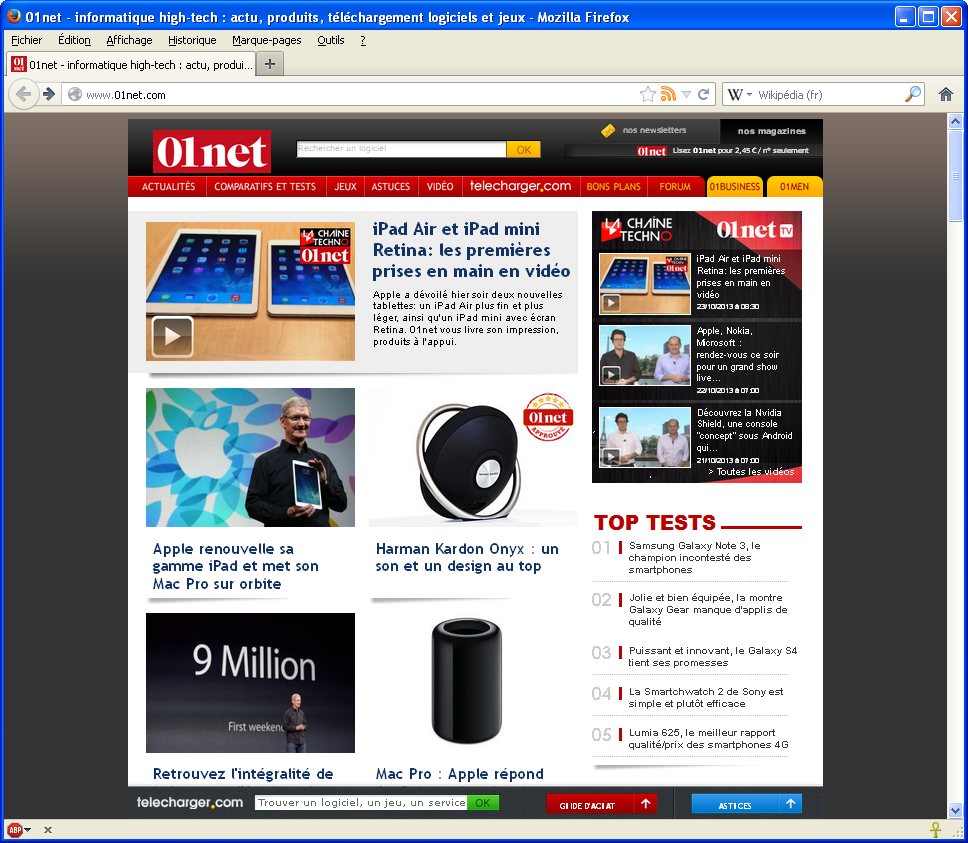
\includegraphics[scale=0.4] {./images/Adblock02.png}
\end{center}
\end{frame}

%----------------------------------------------------------------------------------------
\begin{frame}
\frametitle{Ghostery, Privacy Badger, Noscript...}
Bloque tous les trackers associés au site.
\begin{center}
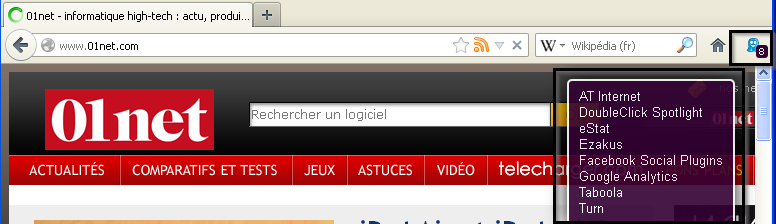
\includegraphics[scale=0.4] {./images/Ghostery_tracker.png}
\end{center}
\end{frame}

%----------------------------------------------------------------------------------------
\begin{frame}
\begin{center}
\Huge{Changer de moteur de recherche}
\end{center}
\end{frame}
%----------------------------------------------------------------------------------------
\begin{frame}
\begin{center}
\frametitle{Duckduckgo - Google tracks you. We don't.}

\url{https://duckduckgo.com}
\\
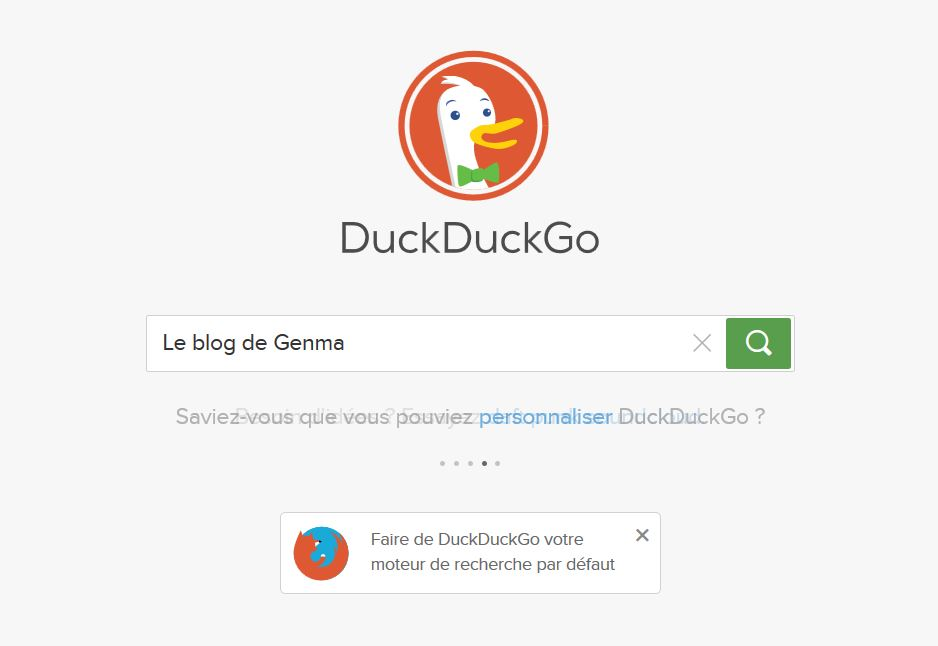
\includegraphics[scale=0.6] {./images/DuckDuckGo.jpg}
\end{center}
\end{frame}

\begin{frame}
\begin{center}
\frametitle{Par Framasoft}

Framabee \url{https://framabee.org} ou TontonRoger \url{https://tontonroger.org/}
\\
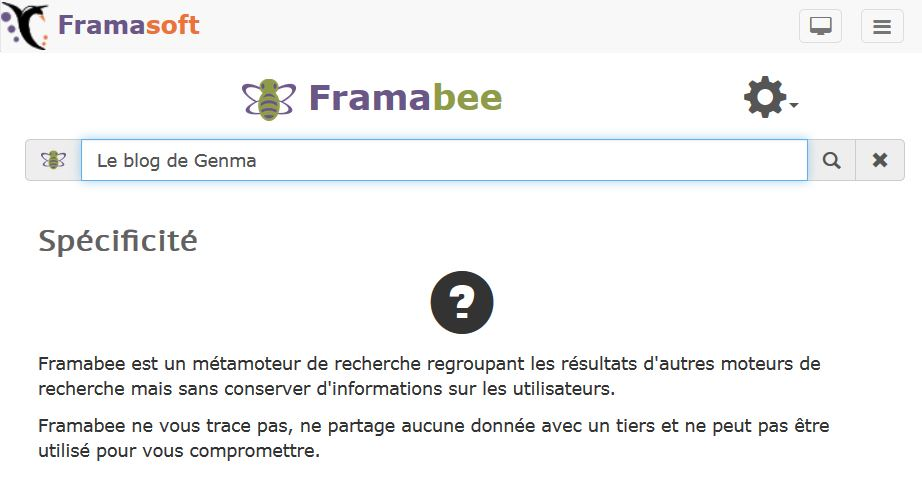
\includegraphics[scale=0.6] {./images/Framabee.jpg}
\end{center}
\end{frame}

\begin{frame}
\begin{center}
\frametitle{Qwant}

\url{https://qwant.com}
\\

\includegraphics[scale=0.6] {./images/Qwant.jpg}
\end{center}
\end{frame}

%----------------------------------------------------------------------------------------
\begin{frame}
\begin{center}
\Huge{Changer de Cloud}
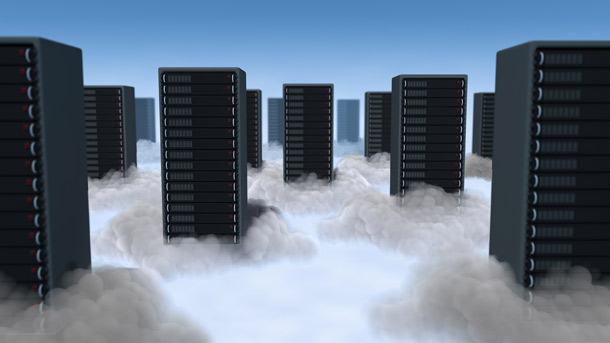
\includegraphics[scale=0.35] {./images/cloud_data_center.jpg}
\end{center}
\end{frame}

\begin{frame}
\begin{center}
\huge{Le cloud c'est l'ordinateur de quelqu'un d'autre, le kloug c'est le gâteau d'un autre. On préfèrera toujours quand c'est le sien.}
\end{center}
\end{frame}


%----------------------------------------------------------------------------------------
\begin{frame}
\frametitle{Des clouds professionnels}
\begin{center}

\includegraphics[scale=0.4] {./images/cloud-orange.png}~

\includegraphics[scale=0.4] {./images/cloud-microsoft.png}~

\includegraphics[scale=0.35] {./images/Google-Cloud-Computing.jpg}
\end{center}
\end{frame}
%----------------------------------------------------------------------------------------
\begin{frame}
\begin{center}
\Huge{Je plaisante, c'est pour voir si vous suiviez...}
\end{center}
\end{frame}

%----------------------------------------------------------------------------------------
\begin{frame}
\begin{center}
\frametitle{Framasoft et tous ses outils de Degogglisons}
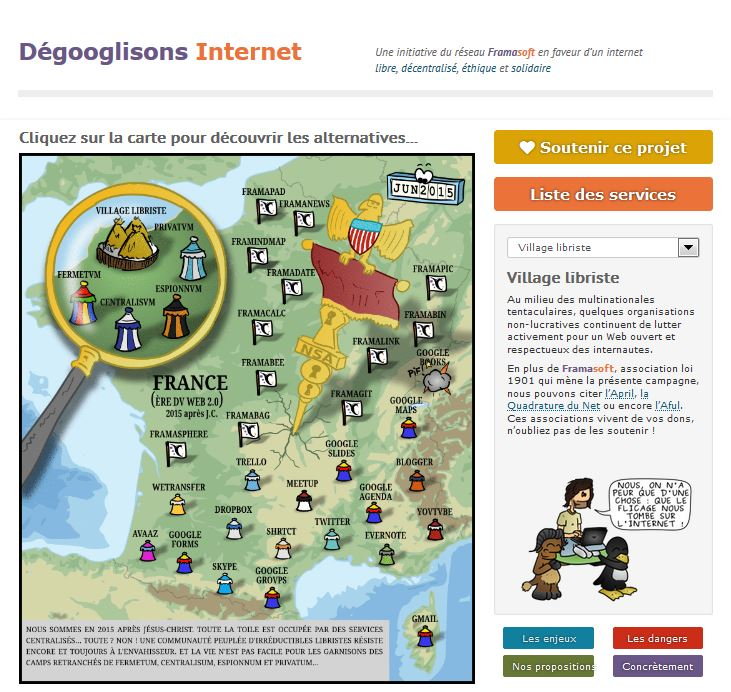
\includegraphics[scale=0.6] {./images/framasoft_degogglisons.jpg}
\end{center}
\end{frame}
%----------------------------------------------------------------------------------------
\begin{frame}
\begin{center}
\frametitle{Cozycloud}
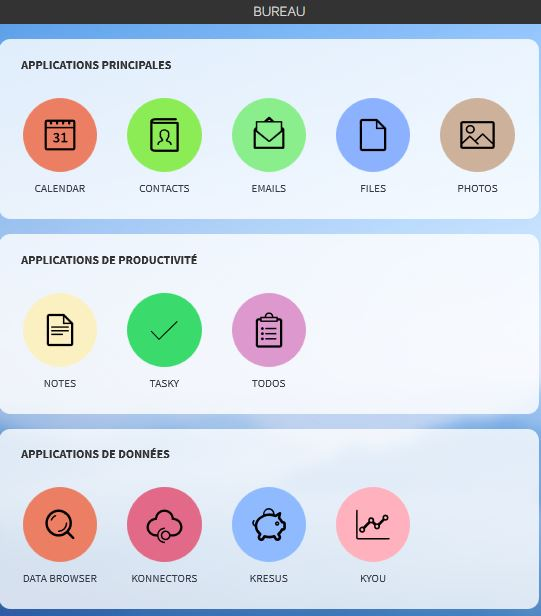
\includegraphics[scale=0.6] {./images/Cozycloud.jpg}
\end{center}
\end{frame}

%----------------------------------------------------------------------------------------
\begin{frame}
\begin{center}
\frametitle{Owncloud}
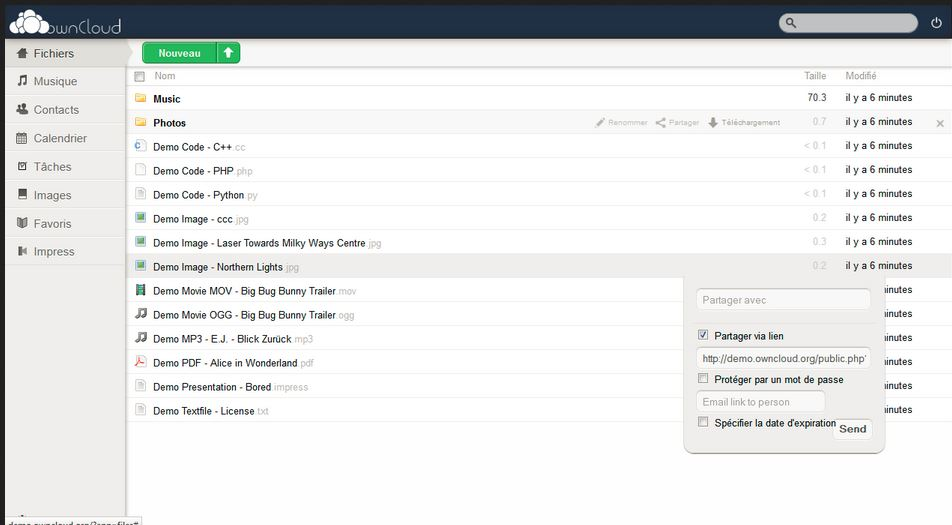
\includegraphics[scale=0.6] {./images/owncloud.jpg}
\end{center}
\end{frame}
%----------------------------------------------------------------------------------------
\begin{frame}
\begin{center}
\frametitle{La brique Internet}
\url{http://labriqueinter.net}
\\~\\
\includegraphics[scale=0.1] {./images/labriqueinternet.png}
\end{center}
\end{frame}

%----------------------------------------------------------------------------------------
\begin{frame}
\begin{center}
\Huge{Tor ? }
\\~\\ 
\includegraphics[scale=0.4]{./images/logo_tor.jpg}
\end{center}
\end{frame}

%----------------------------------------------------------------------------------------
\begin{frame}
\begin{center}
\Huge{Café vie privée, chiffrofête, cryptoparty}
\end{center}
\end{frame}

\begin{frame}
\begin{center}

\includegraphics[scale=0.4] {./images/LogoCafeViePrivee.jpg}
\end{center}
\end{frame}

%----------------------------------------------------------------------------------------
\begin{frame}
\Huge{\centerline{Merci de votre attention.}}
\Huge{\centerline{Place aux questions.}}
\end{frame}

%----------------------------------------------------------------------------------------
\begin{frame}
\frametitle{
\includegraphics[scale=0.4]{./images/Genma.jpg} \ \ \  Me contacter?}
\Huge{\centerline{Le Blog de Genma}}
\Huge{\centerline{http://genma.free.fr}}
\Huge{\centerline{~}}
\Huge{\centerline{Twitter : @genma}}
\end{frame}

%============================================================================================
\end{document}